%%%%%%%%%%%%%%%%%%%%%%% file typeinst.tex %%%%%%%%%%%%%%%%%%%%%%%%%
%
% This is the LaTeX source for the instructions to authors using
% the LaTeX document class 'llncs.cls' for contributions to
% the Lecture Notes in Computer Sciences series.
% http://www.springer.com/lncs       Springer Heidelberg 2006/05/04
%
% It may be used as a template for your own input - copy it
% to a new file with a new name and use it as the basis
% for your article.
%
% NB: the document class 'llncs' has its own and detailed documentation, see
% ftp://ftp.springer.de/data/pubftp/pub/tex/latex/llncs/latex2e/llncsdoc.pdf
%
%%%%%%%%%%%%%%%%%%%%%%%%%%%%%%%%%%%%%%%%%%%%%%%%%%%%%%%%%%%%%%%%%%%


\documentclass[runningheads,a4paper]{llncs}

\usepackage{amssymb}
\setcounter{tocdepth}{3}
\usepackage{graphicx}
\usepackage{color}
\usepackage{amsmath,amssymb,mathtools}
\usepackage{listings}
\usepackage{algorithm}
\usepackage{algorithmic}
\usepackage{centernot}
\usepackage{tikz}
\usetikzlibrary{calc}
\usetikzlibrary{shapes}
\usepackage{pgfplots}
\usepackage{pgfplotstable}


%%%%% BEGIN SPACE SAVERS %%%%%
\usepackage{times} % More compact font, allowed by lncs
\usepackage{microtype} % reduces some unnecessary spaces

% Reduces useless spacing around section headers
\makeatletter
\renewcommand\section{\@startsection{section}{1}{\z@}%
                       {-2\p@ \@plus -4\p@ \@minus -4\p@}%
                       {5\p@ \@plus 2\p@ \@minus 2\p@}%
                       {\normalfont\large\bfseries\boldmath
                        \rightskip=\z@ \@plus 8em\pretolerance=10000 }}
\renewcommand\subsection{\@startsection{subsection}{2}{\z@}%
                       {-8\p@ \@plus -4\p@ \@minus -4\p@}%
                       {4\p@ \@plus 2\p@ \@minus 2\p@}%
                       {\normalfont\normalsize\bfseries\boldmath
                        \rightskip=\z@ \@plus 8em\pretolerance=10000 }}
\renewcommand\subsubsection{\@startsection{subsubsection}{3}{\z@}%
                       {-4\p@ \@plus -4\p@ \@minus -4\p@}%
                       {-1.5em \@plus -0.22em \@minus -0.1em}%
                       {\normalfont\normalsize\bfseries\boldmath}}
\makeatother

% Reduce useless space before paragraphs
\makeatletter
\renewcommand\paragraph{\@startsection{paragraph}{4}{\z@}%
                                      {\parskip}%{3.25ex \@plus1ex \@minus.2ex}%
                                      {-1em}%
                                      {\normalfont\normalsize\itshape}}
\makeatother

% Nuclear weapon: use only if strictly needed :)
%\def\baselinestretch{0.97}

%%%%% END SPACE SAVERS %%%%%


\newcommand\x[1]{\ensuremath{\mathit{#1}}}
\newcommand\lrangle[1]{\ensuremath{\langle#1\rangle}}

\makeatletter
\providecommand{\bigsqcap}{%
  \mathop{%
    \mathpalette\@updown\bigsqcup
  }%
}
\newcommand*{\@updown}[2]{%
  \rotatebox[origin=c]{180}{$\m@th#1#2$}%
}
\makeatother


%\usepackage{url}
%\urldef{\mailsa}\path|{dwyer, mgerrard}@cse.unl.edu|    
%\newcommand{\keywords}[1]{\par\addvspace\baselineskip
%\noindent\keywordname\enspace\ignorespaces#1}

\begin{document}

\mainmatter  % start of an individual contribution

% comment macro
\newcommand{\mycomment}[1]{\textit{\textcolor{red}{#1}}}
\newcommand{\ignore}[1]{}

% first the title is needed
\title{Probabilistic Program Analysis}

% a short form should be given in case it is too long for the running head
\titlerunning{Probabilistic Program Analysis}

\author{Matthew B. Dwyer\inst{1}
\and Antonio Filieri\inst{2}\and Jaco Geldenhuys\inst{4}\and Mitchell Gerrard\inst{1}\and\\
Corina S. P\u{a}s\u{a}reanu\inst{3}\and Willem Visser\inst{4}}
%
\authorrunning{Probabilistic Program Analysis}
% (feature abused for this document to repeat the title also on left hand pages)

% the affiliations are given next; don't give your e-mail address
% unless you accept that it will be published
\institute{University of Nebraska -- Lincoln
\and Imperial College London
\and Carnegie Mellon Silicon Valley and NASA Ames Research Center
\and University of Stellenbosch
}
%Tiergartenstr. 17, 69121 Heidelberg, Germany\\
%\mailsa\\
%\url{http://www.springer.com/lncs}}

%
% NB: a more complex sample for affiliations and the mapping to the
% corresponding authors can be found in the file "llncs.dem"
% (search for the string "\mainmatter" where a contribution starts).
% "llncs.dem" accompanies the document class "llncs.cls".
%

\toctitle{Lecture Notes in Computer Science}
\tocauthor{Authors' Instructions}
\maketitle


\begin{abstract}
This paper provides a survey of recent work on adapting 
techniques for program analysis to compute probabilistic
characterizations of program behavior.  We survey how the
frameworks of data flow analysis and symbolic execution have
incorporated information about input probability distributions
to quantify the likelihood of properties of program states.
We identify themes that relate and distinguish a variety of
techniques that have been developed over the past 15 years
in this area.  In doing so, we point out opportunities for
future research that builds on the strengths of different techniques.
\keywords{data flow analysis, symbolic execution, abstract interpretation, model checking, probabilistic program, Markov Decision Processes}
\end{abstract}

\section{Introduction}
\label{sec:introduction}

Static program analyses aim to calculate properties of 
the possible executions of a program without ever running the program,
and have been an active topic of study for over five decades.
Initially developed to allow compilers to generate more efficient
output programs, by the mid-1970s \cite{fosdick1976data} researchers had
understood that such program analyses could be applied to fault
detection and verification of the absence of specific classes of faults.

The power of these analysis techniques, and what distinguishes them from
simply running a program and observing its behavior, is their
ability to reason about program behavior without knowing all of the
exact details of program execution (e.g., the specific 
input values provided to the program, the set of operating system
thread scheduler decisions).  This tolerance of uncertainty allows analyses
to provide useful information when users don't know exactly how
a program will be used (e.g., when a program is first released, when
embedded systems read sensor inputs from the physical world, or
when it is ported to an operating system with a different scheduler).

Static analyses model uncertainty in program behavior
through the use of various forms of abstraction and symbolic representation.
For example, symbolic expressions are used to encode logical constraints 
in symbolic execution~\cite{king1976symbolic}, to define abstract domains
in data flow analysis~\cite{kildall1973unified,cousot1977abstract}, and to 
capture sets of data values that constitute reachable states via
predicate abstraction~\cite{graf1997predabs}.
Nondeterministic choice is another widely used approach for modeling
uncertainty---for instance, in modeling uncertain branch 
decisions in data flow analysis,
or scheduler decisions in model checking.
While undeniably effective, these approaches sacrifice potentially
important distinctions in program behavior.   

Consider a program that accepts an integer input representing
a person's income.  A static analysis might reason about the program
by allowing any integer value, or, perhaps, by applying
some simple assumption, i.e., that income must be non-negative.
Domain experts have studied income distributions and find that
incomes vary according to a generalized beta distribution 
\cite{mcdonald1984some,thurow1970analyzing}.  Can this type of information be 
exploited to yield useful analysis results when classic
analyses fail, or to reason about new types of program properties?

\ignore{
For decades, there has been a growing awareness of the value of 
incorporating more precise forms of uncertainty into program behavior.  
The field of randomized algorithms has studied how to incorporate
randomness as an additional program input---as a means of achieving
good average case performance, and consequently, as a defense against
intolerable worst case performance.
Programming such algorithms requires that primitives be available
to draw values from probability distributions, and there are many
languages that provide such primitives, e.g., NetLogo \cite{tisue2004netlogo},
the C++ \texttt{$\mathtt{<random>}$} library, and the GNU Scientific library.
}

Whether information about the distribution of
values is embedded within a program or stated as an input assumption,
the semantics of such probabilistic programs is well-understood---and
has long been studied 
\cite{kozen1981semantics,kozen1983probabilistic,jones1990probabilistic,morgan1996probabilistic}
\setcounter{footnote}{0}
\footnote{In recent
years, the term probabilistic program has been generalized beyond
drawing inputs from probability distributions, which we
consider here, to programs that can condition program behavior---by
rejecting certain program runs---and thereby be viewed as
computations over probability distributions.  We refer the reader to the
recent paper by Gordon, Henzinger, Nori and Rajamani \cite{Gordon2014}
for discussion of the analysis of these more general probabilistic programs.}. 
What has lagged behind is the development of frameworks for 
defining and implementing static analysis techniques for such programs.

What would such analyses have to offer?
They can, of course, provide a means of analyzing programs that compute
with values chosen from probability distributions, but they offer much
more.
For example, researchers have explored the use of probabilistic analysis
results to assess the security of software components~\cite{mardziel2013dynamic},
to assess program reliability~\cite{Filieri2013}, to measure program
similarity~\cite{Geldenhuys2012}, 
to characterize the coverage
achieved by an analysis technique~\cite{DwyerASE11}, and to provide information
about program properties when a classic analysis would fail, e.g.,
by running out of memory, time, or due to excessive approximation.

In this paper, we survey work on adapting data flow analysis 
and symbolic execution to use probabilistic information.
We begin with background that provides basic definitions
related to static analysis and probabilistic models.
Section~\ref{sec:overview} attempts to expose some of the key
intuitions and concepts that cross-cut the work in this area.
The following two sections, \ref{sec:pdfa}-\ref{sec:pse}, 
survey work on probabilistic data flow analysis and probabilistic
symbolic execution.  
Section~\ref{sec:computingprobabilities} discusses approaches that
have been developed to reason about the probability of program-related 
events, e.g., executing a path, taking a branch, or reaching a state.
We conclude with a set of open questions
and research challenges that we believe are worth pursuing.


\section{Overview}
\section{Scope and Background}
\label{sec:background}

\ignore{
\begin{enumerate}
\item abstraction refinement
\item fixpoint
\end{enumerate}
}

We focus in this paper on programs that draw input variables
from given probability distributions, or equivalently that make
calls on functions returning values drawn from given distributions
such as those provided by the C++ \texttt{<random>} library.
\mycomment{We should pull an example from one of the later sections
back here to illustrate the idea.}

While researchers have developed analyses that consider a wide
range of program properties, in this survey
we restrict our attention to program
properties that can be encoded as boolean predicates that
can be embedded in the program,
e.g., \texttt{assert} statements, to simplify the explanation
of how probabilities are incorporated into the analyses.
These are refered to as \textit{invariant properties} since
they are intended to hold at every state reached
in all program program executions

\subsection{Programs and Program Analyses}
A program defines a set of execution \textit{traces} each of
which is a sequence of \textit{concrete states}, i.e., 
the current program counter and a map from memory locations to values.
A program \textit{satisfies} an invariant property if in all states in
all traces the predicate evaluates to true, otherwise the program
\textit{falsifies} the property.

A key concept in the program analysis frameworks we survey is
\textit{symbolic abstraction}.  A symbolic abstraction is a 
representation of a set of states.  Abstractions can be encoded
in a variety of forms, e.g., logical formula or binary
decision diagrams \cite{BDD}.  

Analyses that seek to prove the satisfaction of properties generally
define abstractions that \textit{overapproximate} the set of program
states, whereas that seek to falsify properties generally define
abstractions that \textit{underapproximate} the set of program states.

With overapproximating analyses it is common to define an \textit{abstract
domain}, $\mathcal{A}$, 
which symbolically represents a set of concrete states which 
are said to be defined over the \textit{concrete domain}, $\mathcal{A}$.
For any reachable state of a program a pair of abstraction 
and concretization functions, 
$\alpha : \mathcal{C} \mapsto \mathcal{A}$ and  
$\gamma : \mathcal{A} \mapsto 2^\mathcal{C}$,
serve to relate the concrete and abstract domains such that 
$\forall c \in \mathcal{C} : \alpha(c) \in \mathcal{A}$ and $c \in \gamma(\alpha(c))$.
Such an abstract domain is typically partially ordered, $\sqsupseteq$,
such that 
$\forall a,a' \in \mathcal{A} :  a \sqsupseteq a' \implies \gamma(a) \supseteq \gamma(a')$.

Data flow analysis (and abstract interpretation) can be viewed as a
non-standard interpretation of program executions over an abstract
domain.  The semantics of program statements is lifted to operate
on a set of states, encoded as an element of the abstract domain,
rather than a single concrete state.  For a program statement $\tau$,
$\tau^\#$ defines its abstract semantics such that
$\forall c, c' \in \mathcal{C} : \tau(c) = c' \implies \tau^\#(\alpha(c)) \sqsupseteq \alpha(c')$.  This implies the classic overapproximating correctness
relation for abstracted program statements:
$\tau^\# \sqsupseteq \alpha \circ \tau \circ \gamma$.

\mycomment{Matt: add definitions of underapproximation and whatever
else symbolic execution needs}

\mycomment{Matt: develop a figure which shows pseudo code for model checking,
data flow analysis, and symbolic execution side by side}

\mycomment{Matt: walk through an explanation of that figure which
is where we will define what a fixpoint is}

\subsection{Probabilities and Probabilistic Models}
Define and explain the following
\begin{itemize}
\item probability measure
\item rewards/costs
\item discrete time Markov chain
\item discrete time Markov decision process
\end{itemize}


\section{Overview}
\label{sec:overview}

The literature on incorporating probabilistic techniques into 
program analysis is large and growing, technically deep, and quite
varied.  In this paper we cannot hope to cover all of it, but our
intention is to expose key similarities and differences between 
families of approaches and, in doing so, provide the reader with
intuitions that are often missing in the detailed presentation of
techniques, quite helpful in understanding them.

\subsection{Where do the probabilities come from?}

\subsection{What does the analysis compute?}
There are two perspective adopted in the literature.
(1) One can view a probabilistic program as a transformer on probability
distributions and compute the probability distribution, over the
concrete domain, that holds at a program state.
(2) View a probabilistic program as a program whose inputs happen
to vary in some principled way and compute program properties, 
properties of sets of concrete domain elements, along with a characterization
of how that property varies with varying input.

\ignore{
example showing a negation function with drawBernoulli(0.25)
and how it transforms a distribution

show a program that tests whether the absolute value of a number
is greater than 5 where the input is distributed according to N(0,1)
}

Within these there are different approaches taken to estimating
these quantities.  Upper bounds, lower bounds, expectations, ...

\subsection{Handling abstraction expressed through non-determinism}
This cross-cutting theme is addressed in all program analyses that
hope to scale. 

All of the techniques use MDPs and then analyze maximal/minimal
schedules.



\section{Probabilistic Approaches to Program Analysis}
This section introduces probabilistic variants of data flow
analysis and symbolic execution.  Several of these variants
either exploit, or could be adapted to exploit, recent advances in 
methods for quantifying or estimating constraint solution spaces
which we discuss at the end of this section.

\section{Probabilistic Data Flow Analysis}
\label{sec:pdfa}

The key challenge in probabilistic data flow analyses is
determining how probabilities are incorporated into the control
and data abstractions that form its foundation.

\subsection{Control Flow Probabilities}
Early work in extending data flow analysis 
techniques with probabilities did not consider
the semantics of the program. 
Instead user-defined probabilities 
were attached to nodes in the program's control flow graph.  
This allowed the analysis to estimate
the probability of an expression evaluating 
to some value or type at runtime, which could 
allow useful program optimization.

This approach begins with a control flow graph where each edge is 
mapped to the probability that it is taken during execution.
The sum of all probabilities leaving any control flow node must be 1
(excepting the exit node).
These probabilities may be obtained through heuristics, profiling,
or some static analysis.
Imagine an execution trace following some path along the edges of
the control flow graph.
The probability of executing that trace is expressed as the product of 
edge probabilities along this path.
So the probability of executing some program point can be seen as the
summation of the probabilities of traces which can reach that program point.

\begin{figure}[t]
\tikzstyle{every node}=[text width=10em, text centered, font=\scriptsize, inner sep=0pt]
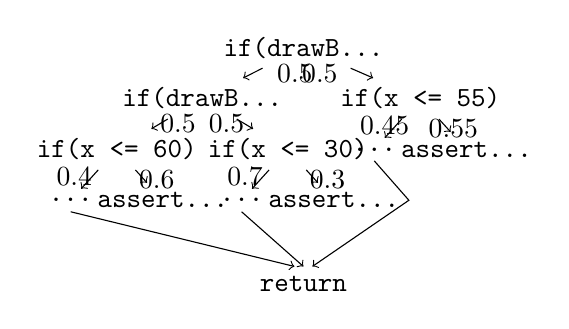
\begin{tikzpicture}[scale=0.38, level/.style={sibling distance = 15mm, level distance = 17mm}]
  \node[yshift=0mm] {\texttt{if(drawB...}}
   child{
    node[xshift=-10mm] {\texttt{if(drawB...}}
     child{
      node[xshift=-8mm] {\texttt{if(x <= 60)}}
       child{
        node[name=e1,xshift=-3mm] {\texttt{...}}
        edge from parent[->] node[left,xshift=12mm] {0.6}
       }
       child{
        node[xshift=3mm] {\texttt{assert...}}
        edge from parent[->] node[right,xshift=-12mm] {0.4}
       }
      edge from parent[->] node[left,xshift=12mm] {0.5}
     }
     child{
      node[xshift=8mm] {\texttt{if(x <= 30)}}
       child{
        node[name=e2,xshift=-3mm] {\texttt{...}}
        edge from parent[->] node[left,xshift=12mm] {0.3}
       }
       child{
        node[name=m1,xshift=3mm] {\texttt{assert...}}
        edge from parent[->] node[right,xshift=-12mm] {0.7}
       }
      edge from parent[->] node[right,xshift=-12mm] {0.5}
     }
     edge from parent[->] node[left,xshift=12mm] {0.5}
   }
   child{
    node[xshift=12mm] {\texttt{if(x <= 55)}}
     child{
      node[name=e3,xshift=-3mm] {\texttt{...}}
      edge from parent[->] node[left,xshift=12mm] {0.55}
     }
     child{
      node[xshift=3mm] {\texttt{assert...}}
      edge from parent[->] node[right,xshift=-12mm] {0.45}
     }
    edge from parent[->] node[right,xshift=-12mm] {0.5}
   }
;
\node[name=r,yshift=-30mm] {\texttt{return}};
\draw[->] (e1.south) to ($(r.north)+(-3mm,0)$);
\draw[->] (e2.south) to ($(r.north)+(0,0)$);
\draw[->] (e3.south) to ($(m1.east)+(0,0)$) to ($(r.north)+(3mm,0)$);
\end{tikzpicture}
\caption{Probabilistic CFG}
\label{fig:prob-cfg}
\end{figure}


Figure~\ref{fig:prob-cfg} shows the probabilistic CFG for the
example from Figure~\ref{fig:example} given that input $x$
is uniformly distributed in the range $[1,100]$.

To compute the probability of a data flow fact holding 
at a program point, Ramalingam uses a slightly
modified version of Kildall's dataflow analysis framework
~\cite{ramalingam1996data}.
Instead of the usual semilattice with an idempotent meet
operation a non-idempotent addition operator is used.
The restricted properties of the meet operation can be
relaxed because instead of computing invariant dataflow
fact, we only want the summation of probabilities of all
traces reaching a certain point.
The expected frequencies may now be computed as the least
fixed point using the same iterative algorithm presented
in the background; the quantity becomes a
{\sl sum-over-all-paths} instead of a {\sl meet-over-all-paths}.

Ramalingam's work assumes execution history does not matter --  
the analysis is path insensitive.
Later work adds some path sensitivity \cite{mehofer2001novel}, 
but as both frameworks deals with exploded control flow graphs, a fully 
path-sensitive approach is not tractable.

Ramalingam's sum-over-all-paths approach is reminiscent of
the approach taken in probabilistic model checking of DTMCs.
In that approach a system of linear equations is formulated
whose solution computes the probability with which a property
holds -- so called \textit{quantitative} properties in 
PRISM \cite{PRISMmarktoberdorf}.   Ramalingam formulates an
equivalent system of linear equations.  

Both of these techniques rely on being able to annotate
branch decisions in the program, or model in PRISM's case, 
with probabilities.  When those decisions are governed by
computed conditions over input variables the calculation of
branch probabilities quickly becomes challenging -- as we will
see in Section~\ref{sec:pse} the techniques from 
Section~\ref{sec:computingprobabilities} can be applied to
this problem.

\ignore{
Accurately estimating control flow probabilities is a significant
challenge, but the techniques from Section~\ref{sec:computingprobabilities}
offer one means of approaching that problem.
}

\subsection{Abstract Data Probabilities}
Within the last 15 years, researchers 
began incorporating probabilistic information directly into
the semantics of a program and then abstracting over 
those semantics \cite{monniaux2000abstract,others}
to enable data flow analysis.
This is typically done using a variation on Kozen's 
probabilistic semantics \cite{kozen1981semantics} 
alongside traditional data flow techniques.
Embedding probabilities into the semantics allows 
the expression of both control and data influences on property
probabilities computed during the analysis.

\subsubsection{Abstracting Probability Distributions}
The first work in this area, by 
Monniaux \cite{monniaux2000abstract,monniaux2001backwards},
developed the key insights that most work in this area has built on. 
The goal is to exploit the rich body of work on developing
abstract domains and associated transformers and extend them
so as to record bounds on probability measures for the concrete values
described by domain elements.

Monniaux's work took the view that probabilistic programs 
effectively transform an input distribution into an output
distribution.  More generally, they compute a distribution that
characterizes each point in the program.   
Here a probabilistic abstract domain, $\mathcal{A}_p$, 
is (an indexed) collection of pairs, $\mathcal{A} \times [0,1]$.
Given a concrete value $c$, 
an upper approximation of its probability 
at a program location with probabilistic abstract domain
value $pa = \{(a_1,w_1), ..., (a_n,w_n)\}$
is given by $\sum_{j \in \{ i \vert (a_i,w_i) \in pa \wedge   
c \in \gamma(a_i)\}} w_j$.   A concrete
value may lie in a number of abstract domains defined by
the probabilistic abstract domain value.  For each such abstract
domain the associated probability \textit{weight} must be totalled
to bound of the probability of the concrete value.

To clarify, these weight components are \textit{not} bounds on the probability
the abstract domain as a whole, but rather they bound the probability
of each concrete element represented by the abstract domain.
This simplifies the formulation of the probabilistic abstract
transformers, i.e., the extension of $\tau^\#$ to account to 
$\mathcal{A}_p$, as discussed below, but it means that additional
work is required to compute the probability of a property holding.
Fundamentally that requires estimating the size of the concretization
of the abstract domain element and then multiplying by the computed bound for
each concrete value.  

Recall that the techniques from 
Section~\ref{sec:computingprobabilities} can be applied to
the problem of counting the concretization of an abstract domain element 
that is encoded as a logical formula.  This may offer a potential
connection between data flow analyses formulated over distributions
and those formulated over abstract states -- which we discuss below.

The design of probabilistic abstract transformers, as with 
classic abstract transformers, can be subtle.
For statements that generate variables drawn from a probability
distribution an upper approximation of the distribution for
regions of the abstract domain is required.  The literature
has constructed these using ad-hoc techniques, but we believe
the methods of Section~\ref{sec:counting} might be applied to 
achieve this and describe this further in Section~\ref{sec:future}.
For sequential statements, weight components are propogated
and abstract domain elements are updated by the underlying transformer.

For conditionals, the transformer can be understood
as filtering the abstract domain between those execution environments which
satisfy the conditional and those which falsify the conditional. 
The difference in the probabilistic abstract environment with weights 
is that the filter is only applied to the first component of
the tuple (the traditional elements of an abstract domain), 
and leaves the weight unchanged.
For instance, consider the abstract domain of an interval of 
integers defined by the tuple, $([-5,5],0.1)$. 
If this domain holds before a conditional of 
{\tt if(x<0)\{...\}}, after applying the filter on the true branch, 
we get $([-5,-1],0.1)$. 
After applying the filter on the false branch, we get $([0,5],0.1)$.
The space is reduced; the weights remain the same.

Finally, reaching fixpoints for rich probabilistic abstract domains
appears to require widening \cite{monniaux2000abstract,esparza2011probabilistic} to be cost-effective.

\subsubsection{Probability for Abstract States}



\mycomment{Matt: discuss Di Pierro's latest work which defines
abstract branch probabilities.}

Bounds on the probability of a state property have been well studied.
Di Pierro et al. \cite{di2013probabilistic} aim to estimate the probability of a property,
rather than bound it.  They formulate their an abstract 
domain over vector spaces, instead of lattices, and use
the Moore-Penrose pseudo-inverse instead of the usual fixed point.
While shown to be effective on small programs, the space
complexity of vector space encodings and lack of tool support
have not yet demonstrated the scalability of the approach.


\subsection{Handling nondeterminism}
When abstraction of program choice are required or when 
there is no basis for defining an input distribution programs,
it is natural to use non-determinism to account for the uncertainty
in program behavior.

In Monniaux's semantics\cite{MonniauxMDP}, choices that can be tied to a known
distribution are cleanly separated from those that cannot.
A nondeterministic choice allows for independent outcomes, and
this is modeled by lifting the singleton outcomes of deterministic
semantics to powersets of outcomes.
In the probabilistic setting, the elements of this powerset are
tuples of the abstract domain and the associated weight, defined
above.  So for any nondeterminstic choice, the resulting computation 
is safely modeled by one of these tuples.  The challenge in the
analysis is to select from among those tuples to compute a useful
probability estimate.

\mycomment{Matt: more here with discussion of original Monniaux work,
add a very short discussion of the 2-player game approach then just
mention these}
\cite{PRISMabstraction,wachter2010best,esparza2011probabilistic}.

\subsection{More and varied probabilistic data flow analyses}
\mycomment{Go through most recent related work and characterize it
here}

More recent work has explored computing an alternative probabilistic
property called {\sl expectation invariants} \cite{chakarov2014expectation}.
This approach uses an iterative data flow analysis to 
compute a bound on the long-run expected value of
some program expression, e.g. $E[f(\mathit{uniform}(0,10))] < 7$ states that,
over a sufficiently large number of runs, when $f$ is called with
a uniformly distributed number in the range $[0,10]$, it will return
an average value less than 7.

The idea of a ``probabilistic program" has been generalized from
Kozen's original semantics to include conditioning on program
observations~\cite{Gordon2014}.
In this setting, the program implicitly specifies a probability 
distribution conditioned on these stated observations.
Data flow analyses have recently been adapted to perform Bayesian
inference on this new class of probabilistic 
programs~\cite{claret2013bayesian}.  

\subsection{Probabilistic Symbolic Execution}
\label{sec:pse}

Probabilistic symbolic execution extends traditional symbolic execution with the ability of computing probabilities of reaching certain traget states in a program.
%executing program paths.
The computation is based on {\em quantifying} the solution spaces of the path conditions computed by symbolic execution.

%Symbolic execution produces path conditions (PCs), i.e., constraints on the inputs, that characterize how a certain target property can be reached. During the process of symbolic execution, the most important question to answer about each PC is whether it is satisfiable or not.  If not, then the corresponding path does not need to be analyzed any further.  However, now we are additionally interested in the \emph{probability} of a target property being satisfied. 

%For simplicity, we assume we are working with a uniform input distribution for the program under analysis.  
%See \cite{Filieri2013} for a detailed discussion of input distributions within symbolic execution.

We illustrate probabilistic symbolic execution using the example in Figure~\ref{fig:symex:illus}, where 
we introduce variables $b_0$ and $b_1$ to model 
the two {\tt drawBernoulli} distributions from Figure~\ref{fig:example};
the domains of those variables consist of 10 values and the tests
check for half of the domain, corresponding to the 0.5 parameter
in the Bernoulli distribution.
Note that this program now has 3 inputs and an input domain size of
$10 \times 10 \times 100 = 10000$.
\ignore{
As in Section~\ref{sec:computingprobabilitiesExact}, $D$ represents the finite discrete domain of the variables.
}
The domain of variables, which is finite and discrete, is denoted by $D$.
Figure~\ref{fig:symex:illus} illustrates the six symbolic paths generated by a symbolic execution of the example program. 
The path condition describing each path is the conjunction of the constraints along the path; for example the leftmost path will have $b_0 < 5 \wedge b_1 < 5 \wedge x \le 60$ as its path condition. 

\begin{figure}[t]
\begin{minipage}{0.3\textwidth}
%\begin{algorithmic}
%  \STATE $\triangleright\quad b_0,b_1\in\{0,\ldots,9\}$
%  \IF{$b_0<5$}
%    \IF{$b_1<5$}
%      \IF{$x\le60$} \STATE $\ldots A$
%      \ELSE \STATE \textbf{assert} \FALSE
%      \ENDIF
%    \ELSE
%      \IF{$x\le30$} \STATE $\ldots B$
%      \ELSE \STATE \textbf{assert} \FALSE
%      \ENDIF
%    \ENDIF
%  \ELSE
%    \IF{$x\le55$} \STATE $\ldots C$
%    \ELSE \STATE \textbf{assert} \FALSE
%    \ENDIF
%  \ENDIF
%\end{algorithmic}
\centering
\footnotesize
\begin{lstlisting}[language=Java,basicstyle=\scriptsize\ttfamily]
// b0, b1 in 0..9
m(int x, int b0, int b1) {
 if(b0<5) {
  if(b1<5) {
   if(x <= 60)
    ...A
   else
    assert false
  } else {
   if(x <= 30)
    ...B
   else
    assert false
  }
 } else {
  if(x <= 55)
   ...C
  else
   assert false
 }
}
\end{lstlisting}
\end{minipage}
\begin{minipage}{0.6\textwidth}
\def\llabel#1{\makebox(0,0)[r]{\small\strut#1\space}}
\def\rlabel#1{\makebox(0,0)[l]{\small\strut\space#1}}
\def\nlabel#1{\begin{picture}(0,0)%
  \put(0,0){\circle{10}}\put(0,0){\makebox(0,0){\small#1}}\end{picture}}
\def\mlabel#1{\begin{picture}(0,0)%
  \put(0,0){\circle{14}}\put(0,0){\makebox(0,0){\small#1}}\end{picture}}
\begin{picture}(250,260)%\put(0,0){\framebox(250,260){}}%
  \put(140,240){\begin{picture}(0,0)
    \put(0,0){\nlabel{1}}
    \put(-3.00,-4.00){\line(-3,-4){54.00}}
    \put(-15,-20){\llabel{$b_0<5$}}
    \put(-25,-32){\llabel{$5000$}}
    \put(-60,-80){\begin{picture}(0,0)
      \put(0,0){\nlabel{2}}
      \put(-2.24,-4.47){\line(-1,-2){35.53}}
      \put(-10,-20){\llabel{$b_1<5$}}
      \put(-17,-32){\llabel{$2500$}}
      \put(-40,-80){\begin{picture}(0,0)
        \put(0,0){\nlabel{3}}
        \put(-1.21,-4.85){\line(-1,-4){17.09}}
        \put(-5,-20){\llabel{$x\le60$}}
        \put(-7,-32){\llabel{$1500$}}
        \put(-20,-80){\mlabel{$A$}}
        \put(1.21,-4.85){\line(1,-4){17.09}}
        \put(5,-20){\rlabel{$x>60$}}
        \put(7,-32){\rlabel{$1000$}}
        \put(20,-80){\mlabel{$A'$}}
        \end{picture}}
      \put(2.24,-4.47){\line(1,-2){35.53}}
      \put(10,-20){\rlabel{$b_1\ge5$}}
      \put(17,-32){\rlabel{$2500$}}
      \put(40,-80){\begin{picture}(0,0)
        \put(0,0){\nlabel{4}}
        \put(-1.21,-4.85){\line(-1,-4){17.09}}
        \put(-7,-30){\llabel{$x\le30$}}
        \put(-9,-42){\llabel{$750$}}
        \put(-20,-80){\mlabel{$B$}}
        \put(1.21,-4.85){\line(1,-4){17.09}}
        \put(7,-30){\rlabel{$x>30$}}
        \put(9,-42){\rlabel{$1750$}}
        \put(20,-80){\mlabel{$B'$}}
        \end{picture}}
      \end{picture}}
    \put(3.00,-4.00){\line(3,-4){54.00}}
    \put(15,-20){\rlabel{$b_0\ge5$}}
    \put(25,-32){\rlabel{$5000$}}
    \put(60,-80){\begin{picture}(0,0)
      \put(0,0){\nlabel{5}}
      \put(-1.21,-4.85){\line(-1,-4){17.09}}
      \put(-5,-20){\llabel{$x\le55$}}
      \put(-12,-32){\llabel{$2750$}}
      \put(-20,-80){\mlabel{$C$}}
      \put(1.21,-4.85){\line(1,-4){17.09}}
      \put(5,-20){\rlabel{$x>55$}}
      \put(12,-32){\rlabel{$2250$}}
      \put(20,-80){\mlabel{$C'$}}
      \end{picture}}
    \end{picture}}
\end{picture}
\end{minipage}
\caption{Illustration of probabilistic symbolic execution}
\label{fig:symex:illus}
\end{figure}

%To compute the probabilities of path conditions, we use a quantification procedure for the generated constraints. In~\cite{filieri2013reliability} we use model counting techniques; libraries such as LattE~\cite{deloera2012software}, algorithmically calculate the exact number of points inside a bounded (possibly very large) region described by linear constraints over a discrete domain.  In more recent work~\cite{borges2014compositional}, we develop quantification procedures for the analysis of programs that have mixed integer and floating point constraints of arbitrary complexity.

%To use model counting techniques to compute the probability $\x{Pr}(\x{pc})$ of path condition \x{pc}, we define a counting function, $\sharp(\x{pc})$, that returns the number of elements of $D$ that satisfy $\x{pc}$. Because we assume that $D$ is finite and countable, $\sharp(\cdot)$ always produces a finite non-negative integer, and $\x{Pr}(\x{pc})$ is, by definition~\cite{pestman1998mathematical}, $\sharp(\x{pc}) / \sharp(D)$ (where $\sharp(D)$ is the size of the non-empty input domain). 

%\subsubsection{Algorithm}

%We outline a general algorithm to probabilistic symbolic execution
%that accomodates many of the advances in the recent literature~\cite{filieri2014statistical,Filieri2013}.
Algorithm {\em pse} (Algorithm~\ref{alg-pse}) illustrates probabilistic symbolic execution;
it is a modification of traditional symbolic execution to process symbolic paths one at a time using procedure {\em symsample}.
The selection of each path can be done systematically (e.g. using depth-first search as in traditional symbolic execution) or statistically, 
guided by branch probabilities as in~\cite{filieri2014statistical}. 
Our description accomodates many of the advances in the recent literature~\cite{filieri2014statistical,Filieri2013}.
The processing of each path involves the calculation of probabilities as described in
the next section.

%Below we discuss in detail procedures \x{stoppingPath}, \x{selectBranch}, \x{stoppingSearch} and \x{processPath} used in the algorithm. 
At a high level, procedure \x{symsample} is called from the initial state of the program; %with $pc=\mathtt{true}$ as the current path condition;  
it returns a single path which is then processed.  After each path, procedure \x{stoppingSearch} is called to check if the analysis is complete or some other termination criterion is met, 
and the analysis can stop. Within procedure \x{symsample} we first check if the search for a path needs to be stopped; otherwise, we symbolically execute the program up to the next branching 
point and decide which of the next branching statements must be taken. 
%Note that in our description, only one branch is taken, 
%unlike in traditional symbolic execution, where both branches could be taken if they were both satisfiable. 

\begin{minipage}{0.4\textwidth}
\begin{algorithm}[H]
\floatname{algorithm}{Alg.}
\caption{\x{pse}$(l,m,pc)$}
\label{alg-pse}
\begin{algorithmic}
 \REPEAT
  \STATE $p \gets \x{symsample}(l_0, m_0, \x{true})$
  \STATE $\x{processPath}(p)$
 \UNTIL {$\x{stoppingSearch}(p)$}
\end{algorithmic}
\end{algorithm}
\end{minipage}
\begin{minipage}{0.55\textwidth}
\begin{algorithm}[H]
\floatname{algorithm}{Alg.}
\caption{\x{symsample}$(l,m,pc)$}
\label{alg-symsample}
\begin{algorithmic}
 \IF{$\x{stoppingPath}(pc)$} 
 \RETURN $pc$
 \ENDIF
 \WHILE{$\neg branch(l)$}
   \STATE $m \gets op(l)(m)$
   \STATE $l \gets succ(l)$
 \ENDWHILE
 
 
 \STATE $c \gets \x{cond}(l)(m)$
 
 \IF{$\x{selectBranch}(c,pc)$}
   \RETURN \x{symsample}$(\x{succ_t}(l), m, pc \wedge c)$
 \ELSE
   \RETURN \x{symsample}$(\x{succ_f}(l), m, pc \wedge \neg c)$
 \ENDIF
\end{algorithmic}
\end{algorithm}
\end{minipage}

$\newline$

\paragraph{Procedure stoppingPath} uses a stopping criterion (limit on search depth) to avoid exploration of infinite or very long paths, that are due to loops conditioned on input variables.
Since some paths might now be truncated before reaching a target property, we introduce three types of paths, (1) {\em success} paths, which reach and satisfy the target property, (2) {\em failure} paths, 
which reach and falsify the property, and (3) {\em grey} paths, which are truncated before reaching the property. These paths form three disjoint sets; we calculate the cumulative probability of success  
$Pr(\x{success})$ (i.e., the {\em reliability} of the code), failure  $Pr(\x{failure})$ and grey paths $Pr(\x{grey})$.  Grey paths can be handled optimistically (grouped with the success paths), pessimistically (grouped with the failure paths) or kept separate and be used as a measure for how confident we are in our estimates (for example, if the grey paths probability is very low, we are more confident). 

\paragraph{Procedure selectBranch} selects which branch to execute next; this can be done either systematically or probabilistically, 
% In the context of symbolic execution, we define a sample as the
%simulation of one symbolic path. Whenever a branch is encountered during such simulation, the decision to proceed along either of the alternative branches has to be taken 
according to the probability of satisfying the corresponding branch conditions. This is computed based on the number of solutions for each path condition as follows.
At each branching point, we count the number of solutions for the path condition at that branching point ($\sharp(pc)$) and the number of solutions for the path condition for both branches ($\sharp(pc \wedge c)$ and $\sharp(pc \wedge \neg c)$). Assuming a uniform distribution of the inputs, the probability for the true branch is then simply  $Pr(\x{succ_t}(l)) = \sharp(pc \wedge c)/\sharp(pc)$; similarly
for the false branch, $Pr(\x{succ_f}(l)) = \sharp(pc \wedge \neg c)/\sharp(pc)$.  Techniques for counting the number of solutions are discussed in Section~\ref{sec:computingprobabilities}.

In the example of Figure~\ref{fig:symex:illus}, when we sample probabilistically at node $3$, we have that the path condition at the node is $pc = b_0 < 5 \wedge b_1 < 5$ and $\sharp(pc) = 2500$. 
The true branch ($b_0 < 5 \wedge b_1 < 5 \wedge x \le 60$ with a count of $1500$) will thus be taken with probability $1500/2500 = 0.6$ and the false branch will be taken with probability $0.4$.  

\paragraph{Procedure processPath} calculates the probability for the path being processed and checks whether the path falls into the success, failure or grey set. Note that many of these calculations have already been performed during the {\tt selectBranch}, and caching can be used to eliminate redundant work. 

Again in the example of Figure~\ref{fig:symex:illus}, the paths ending at the labels $A', B'$ and $C'$ indicate assertion failures, and thus the probability of failure will be $1500/10000 + 1750/10000 + 2250/10000 = 0.55$.  Since there are no loops in the example, the rest of the paths indicate success, which will have probability $0.45$.

Furthermore, the procedure can handle sampling without replacement---to guarantee an exhaustive analysis even when certain behaviors have very small probability. 
In~\cite{filieri2014statistical} we describe how we leverage the counts we store for each path condition to ensure no path is sampled twice. Whenever a path has been explored completely, 
we subtract the final path condition count from all the counts along the current path back up to the root. Note that these counts are being used by \x{selectBranch} to calculate the conditional probabilities at a branch, and thus they change with each sample. If a count becomes zero, the corresponding branch will no longer be selected. The more paths of the program are analyzed, 
the more counts propagate up the tree until the root node's count becomes zero, at which point all paths have been explored. 

\paragraph{Procedure stoppingSearch} uses either a measure of confidence based on the percentage of the input domain that has been explored, or it uses a statistical measure of confidence. 
Enough confidence exists about the portion of the input domain that has been analyzed when  $1 - Pr(\x{success}) + Pr(\x{failure}) < \epsilon$.  If we treat grey paths separately, this means $Pr(\x{grey}) < \epsilon$. The parameter $\epsilon$ is provided by the user, and is typically very small. Note that although we show, for simplicity, that procedure \x{stoppingSearch} 
takes the path as input, in practice it just reuses the results computed by procedure \x{processPath}. 


\subsubsection{Handling nondeterminism}

Handling nondeterminism within the systems being analyzed has been studied in previous work \cite{Filieri2013} in the context of scheduling choices in concurrent programs. The approach was to determine the schedule giving the highest (or lowest) reliability. More recently, an approach based on value iteration learning was presented \cite{luckow2014exact} to handle the problem in a more general fashion.

\ignore{
\subsubsection{More and varied probabilistic symbolic execution}

Probabilistic symbolic execution was introduced in \cite{Geldenhuys2012}, where the approach was to do model counting (using LattE) on-the-fly during symbolic execution. This work was extended in \cite{Filieri2013} to collect path conditions from symbolic execution and then calculate the reliability of the code. This work also showed how input distributions can be handled. In both works it is important to observe that {\it all} paths of the program are analyzed, and thus the probability calculations are precise. 

The work in \cite{Sankaranarayanan2013} was the first to apply sampling of paths during static analysis to provide a probability calculation with a certain confidence bound. They applied the approach to calculate bounds on the probability of assertions holding in the code. In \cite{filieri2014statistical}, an approach similar to Algorithm~\ref{alg-pse} was used to also sample paths and then use Bayesian estimation and hypothesis testing. This paper also introduced the subtraction of the counts to ensure rare events can be sampled (see {\tt processPath} above). 

\mycomment{Anto: the next paragraph will be updated after completing sect 3}
Another important dimension to consider is how to count the solutions for constraints in various domains. The work so far described has mostly focussed on linear integer arithmetic, since the theory is decidable and thus often used as the basis for symbolic execution tools. Fortunately, as already mentioned, efficient model counters also exist for this domain (such as LattE\cite{deloera2012software} and Barvinok\cite{verdoolaegesoftware}). In \cite{Borges2014} non-linear and bounded floating-point domains are handled giving accurate estimates of the size of the solution space. Counting the solutions to constraints complex data-structures, such as objects in Java, are addressed in \cite{Filieri2015}. New domains such counting the solutions to string domains \cite{Aydin2015} and the more general all solutions to a SAT formula (\#SAT) \cite{Chakraborty2014} has recently been proposed. 
}


\section{Computing Program Probabilities}
\label{sec:computingprobabilities}

\mycomment{Matt: it would be good if there was some discussion about
how to handle a given distribution.  For example, how would prob
sym exe handle a call to a function to return a value from N(0,1)
(a normal distribution with mean 1 and standard distrubution 0).
Equivalently how would this be specified as a usage profile.
Is there something better than relying on a person to write this down?
I know there is tons of work published on this, but is there a simple
approach we can describe or that you've used.}


Computing probabilities for probabilistic program analysis can usually be reduced to computing the probability of satisfying a boolean constraint over the program variables. In this section we will introduce some of the basic techniques currently used in program analysis. 

To simplify the notation, we will focus on implicit probabilistic constructs, assuming the program under analysis has input variables $V=\{v_1, v_2, \dots, v_n\}$, where $v_i$ has domain $d_i$ and comes with a probability distribution $\mathcal{P}_i: d_i \to [0, 1]$. The input domain $D$ is defined as the cartesian product of the domains $d_i$, while the input distribution $\mathcal{P}$ is defined as the joint distribution over all the input variables $\prod_i \mathcal{P}_i(\bar{v_i})$. Given a constraint $\phi: V \to \{true, false\}$, our goal is to compute the probability $Pr(\phi)$ of satisfying $\phi$ given the input domains and probability distributions. This problem is usually referred to as model counting, when the input domains are countable, or solution space quantification, when the input domains are modeled as uncountable (e.g., abstracting floating-point numbers as reals).

\mycomment{Anto: Section outline to be added}

\mycomment{Anto: check definitions of model counting and solution space quantification}


%Some techniques allow for bounding the probability value within a certain interval; 

\subsection{Exact and numeric computation}\label{sec:computingprobabilitiesExact}

% OUTLINE
%	\begin{enumerate}
%		\item Finite domains
%			\begin{enumerate}
%				\item Linear integers (Latte, Barvinok, Omega for negation; used in our works)
%				\item Strings (bounds: \url{http://www.comp.nus.edu.sg/~shweta24/publications/smc\_pldi14.pdf} ; automata-based exact and upperbounds: \url{http://www.cs.ucsb.edu/~bultan/publications/model-counting.pdf}; we should also check the related work thereof)
%				\item Data structures (icse13 and spin15)
%				\item Sat and smt (\url{http://arxiv.org/pdf/1306.5726v3.pdf}, \url{http://arxiv.org/pdf/1411.0659.pdf}; these papers should have been published, we should check related work in there)
%			\end{enumerate}
%		
%		\item Uncountable domains
%			\begin{enumerate}
%				\item Symbolic and numerical integration (interesting, but symbolic does not scale apart from a few simple cases, while numeric suffers for large cardinality of input domains; however: general, available off-the-shelf, parallelizable for numerical)
%			\end{enumerate}
%	\end{enumerate}

\paragraph{Finite domains.} 

If the input domain is finite, classic probability can be used to reduce the computation of $Pr(\phi)$ to a counting problem (here we assume a uniform distribution over all the possible input values, i.e., each valid input has the same probability):
%
\begin{equation}\label{eq:counting}
	Pr(\phi) = \frac{\sharp(\phi \land D)}{\sharp(D)}
\end{equation}
%
\noindent where $\sharp(\cdot)$ counts the number of inputs satisfying the argument constraint, $D$ has been overloaded to represent the finite domain as a constraint ($\sharp(D)$ is a short form for the size of the domain)\footnote{More precisely, Equation~\eqref{eq:counting} represents the probability of satisfying the constraint $\phi$ conditioned to the fact that the input is within the prescribed domain $D$.}. For example, considering a single integer input variable $x$ taking values between $1$ and $10$ uniformly, $\sharp(D)=10$ and $\sharp(x\leq5 \land D)=5$, leading to a probability of $.5$ of satisfying the constraint.

Efficient implementations of $\sharp(\cdot)$ are available for several classes of model counting problems:

\begin{itemize}
	\item \textbf{Linear integer arithmetic}: the conjunction of linear constraints over a finite integer domain geometrically defines a multi-dimensional lattice bounded by a convex polytope~\cite{de2008computationalGeometry}. To count the number of points composing this structure, an efficient solution has been proposed by Barvinok in~\cite{barvinok1994polynomial}. This algorithm is grounded on the construction of generating functions suitable for solving the counting problem in polynomial time with respect to the number of variables and the number of constraints. Notably, besides the number of bits required to represent the numerical values, the complexity of this algorithm does not depend on the actual size of the variable domains. This makes the computation feasible for very large input domains, allowing its application to probabilistic program analysis. Several implementations of this algorithm are available, the two most popular being LattE~\cite{LattESoftware} and Barvinok~\cite{verdoolaegesoftware}. When disjunctions appear in the constraint, these have to be preprocessed before applying Barvinok's algorithm (e.g., using the Omega library~\cite{Omega1996}). This normalization increases the overall complexity of model counting, however, several optimizations can be leveraged to reduce the computational effort (we will discuss some later in Section~\ref{sec:computingprobabilitiesOptimizations}). Barvinok's algorithm has been used for probabilistic program analysis in \cite{Geldenhuys2012,Filieri2013,Filieri2015}.

	\item \textbf{Bounded data structures}: data structures are usually composed by a structural dimension, e.g., lists or tree, and by a payload stored in each node of the structure. The level of decoupling between structure and payload differs case by case -- for example, a list of integers may be sorted or not. Early work on complexity analysis explored the use of generating functions for representing the number of valid instances of a given data structure without explicitly enumerating them (e.g.,~\cite{flajolet1985mathematical}). However, despite its computational efficiency, this approach requires a significant amount of human work because the construction of these generating functions can hardly be automatized from source code. For the sake of generality, early work in probabilistic program analysis~\cite{Filieri2013} used enumeration-based approaches, such as Korat~\cite{Korat2002}. This technique relies on the formalization both of the invariants characterizing the valid structures and of the constraints to be counted as executable boolean methods, and then generates all the instances for which these methods return true. The generation is enhanced with smart pruning techniques to reduce the actual exploration space, although their complexity still leaves most realistic programs out of reach. A recent approach proposed in~\cite{Filieri2015} decouples the structural part from the payload, employing the partial enumeration of the former and the use of more efficient model counting techniques for the latter, whenever possible. For example, an acyclic sorted list of integers between 1 and 10 having at most 3 elements would require the enumeration of 4 different structural configuration (including the empty list) and the evaluation of 8 linear integer constraints (which can be computed with Barvinok's algorithm), instead of exploring all 1111 possible instances.

	\item \textbf{Regular expressions}: a variety of practically relevant constraints on strings can be formalized as matching with a regular expression~\cite{Luu2014,Aydin2015}. If the (maximum) length of the string is bounded, the number of instances matching a regular expression can be counted exactly with an automata-based approach. The regular expression is first transformed into the corresponding accepting automata. Then, an exponential generating function is automatically constructed to count the accepting runs of the automata up to a certain length, without the need to enumerate all of them explicitly. The technique is actually more general and can be used for any constraint whose satisfaction can be reduced to counting the accepting runs of a finite state automata. For more general constraints, called pseudo-relational, the exact count is not computable, though its value can be bounded in a finite interval, allowing, in some cases, for best- or worst-case analysis~\cite{Aydin2015}.
	
	\item \textbf{SAT and SMT}: \mycomment{TBD (\url{http://arxiv.org/pdf/1306.5726v3.pdf}, \url{http://arxiv.org/pdf/1411.0659.pdf}; these papers should have been published, we should check related work in there)}

\end{itemize}


\paragraph{Floating-point numbers.} 
Floating-point numbers are usually abstracted as real numbers for analysis purposes. Computing the probability of satisfying a constraint over reals requires refining Equation~\ref{eq:counting} to cope with the density of the domain. In particular, the counting function $\sharp(\phi)$ has to be replaced by the integration of an indicator function on $\phi$, i.e., a function returning $1$ for all the inputs satisfying $\phi$ \cite{Borges2014}. This integration can be performed exactly only for a limited number of cases, where symbolic integration is possible. For all the other cases, only numerical integration is possible. A number of commercial and open-source tools can be used for this purpose, however, 1) numerical computations are accurate only up to a certain bound, and 2) they do not scale when the cardinality of the input domain grows. In the latter case, sampling-based methods are preferable. 

\paragraph{Handling input distributions.} 
For finite domains, we assume, without loss of generality, the input distribution to be specified on a finite partition $D^1, D^2, \dots, D^n$ of the input domain $D$ (i.e., $\cup_i D^i \equiv D$ and $D^i \cap D^j \neq \emptyset \implies i=j$) via the probability function $Pr(D^i)$. We assume elements within the same set $D^i$ to have the same probability. The case of uniform distribution described so far corresponds to the partition with cardinality 1, i.e., the whole domain.
 
Since the elements of the partition are disjoint by construction, we can exploit the law of total probability to extend Equation~\eqref{eq:counting} to include the information about the input distribution:
%
\begin{equation}\label{eq:countingInputDistribution}
	Pr(\phi) = \sum_i \frac{\sharp(\phi \land D^i)}{\sharp(D^i)} \cdot Pr(D^i)
\end{equation}
%
\noindent where $D^i$ has again been overloaded to represent the constraint of an element belonging to $D^i$.

Formalizing the input distribution on a finite partition of the input domain is general enough to capture every valid distribution on the inputs, including possible correlations or functional dependencies among the input variables. However, the finer the specification of the input distribution, the more complex the computation of Equation~\eqref{eq:countingInputDistribution}, which, in the worst case, may require the computation of $|D|$ summands \cite{Borges2014}. While this worst case is unlikely to occur (also due to the optimization strategies that will be described later), more efficient probability computations are possible employing distribution-aware sampling-based methods, which will be described in the next section.

\subsection{Sampling-based methods}\label{sec:computingprobabilitiesSampling}

	\begin{itemize}
		\item Sampling from uniform distributions (base case, best we can if no input distribution is available; based on classic probability, i.e., count success over total)
		\item Discretization of non-uniform distributions (useful when a finite number of usage scenarios are available; can approximate any distribution with arbitrary accuracy; most straightforward when inferring distributions from past executions, i.e., histograms; it does not scale for fine-grained approximations)
		\item Distribution-aware sampling (quite straightforward for distributions over numerical domains; requires more complex, unbiased, input generation techniques when sampling from other domains, e.g., data structures, but similar to random testing; scalability issues when sampling correlated input variables)
      
		\item Monte Carlo methods
			\begin{itemize}
				\item Hit or miss Monte Carlo
				%\item \mycomment{Anto: Mention Crude montecarlo for integration? Gibbs and MCMC sampling will be just mentioned; especially MCMC is used by the MSR guys}
				\item Frequentist and Bayesian estimators (used in prob. model check.)
					\begin{itemize}
						\item historically frequentist first, with static bounds (based on Chernoff's) for prob MC; then sequential ratio tests, still frequentist.
						\item Bayesian from CMU
					\end{itemize}
				\item The variance issue and convergence acceleration techniques (just a paragraph with some refs):
					\begin{itemize}
						\item Importance sampling (used in prob. model check.)
						\item Importance slicing (used in prob. model check.)
					\end{itemize}

				\item Exploiting he law of total probability for composing different estimators: Interval constraints propagation (PLDI14) and statistical/exact (FSE14)
				\item Dealing with nondeterminism (freq and bayesian in prob MC, ASE14)	
			\end{itemize}
			
			\item approximate $\sharp$-sat and $\sharp$-smt (\url{http://arxiv.org/pdf/1306.5726v3.pdf}, )
	\end{itemize}





\subsection{Optimizations}\label{sec:computingprobabilitiesOptimizations}

Divide and conquer from icse13 and and sensitivity-aware sampling from fse15

%\section{Specifying and Inferring Probability Distributions}
\label{sec:probspecs}

The probabilistic symbolic execution defined in the previous section
makes use of a probabilistic {\em usage profile} which is an estimate
of the probability distribution of a program's input space.  Usage
profiles can be {\em specified} based on physical phenomena, known
sensor parameters or other domain specific knowledge about the program
and its deployment context.  They can also be {\em built}
automatically based on observed data from past usages of the program.
Finally, best(worst)-case usage profiles can be {\em inferred} from
the structure of a program itself.  

\subsubsection{Building usage profiles from observed data}
It is possible to obtain usage profiles systematically from
telemetry data, log files and simulation
data available from previous or similar usages (missions) of 
the software under analysis.
For example, one can measure
the frequency of values occurring within certain ranges
during a mission to obtain realistic usage profiles. 
Furthermore, as in the case of Probabilistic
Programming~\cite{gordon-etal-icse-fose2014}, the code can also be
used to formalize the dynamics of a system, from biological processes
to financial markets. In these cases probabilistic profiles can be
either inferred through the analysis of experimental or historical
data or deduced by physical laws.


In the simplest case, operational profiles can be inferred from raw
data by measuring the frequency or proportion of the observed data
within pre-specified ranges.  This gives an estimation of the
distribution of the data for the duration the system was observed.
Such profiles can then be used for a new version or a similar system,
to assess its probabilistic properties.

In addition to the usage profiles that specify the distributions of
the input data~\cite{ICSE13}, one can use stateful usage profiles
given as Discrete-Time Markov Chains (DTMC), for example.  Such
profiles are useful for the class of systems that typically operate on
sequences of inputs -- so called reactive programs.

To apply probabilistic analysis to such systems one must extend both
the usage profiles and the probability computation to consider input
values and probability distributions that are correlated with previous
inputs in the environment.  Conceptually, the DTMC generates a
\textit{driver} that interacts with the analyzed software according to
the distribution.

Informally, DTMC are automata labeled with outgoing probabilities on
their transitions.  DTMC are already a common formalism for expressing
probabilistic usage models and we will employ inference procedures to
build them automatically.  Such inference was presented in
e.g. \cite{GhezziICSE14, Beschastnikh11}). It consumes logged data
which typically consists of a time series; each step encodes the value
of the states observed at each time step. The states of the inferred
model then represent ``abstractions'' of the state reported in the log
file and transitions in the model correspond to the time steps in the
log file. The abstraction is defined by the user and it depends on the
properties of interest. The log data is discretely sampled, in some
cases many times per second, therefore it is necessary to select a
resolution to allow for more realistic state transitions and to
prevent state space explosion. The probability distribution for a
particular state $s$ is estimated by computing the ratio between the
number of traversals for each outgoing transition and the total number
of traversals of the transitions exiting state $s$; this corresponds
to the {\em maximum likelihood estimator} for the probability
distribution at that state.

An alternative is to explore Bayesian inference -- a method of
statistical inference in which Bayes' rule is used to update the
probability estimate for a hypothesis as additional evidence is
acquired. Bayesian updating is an important technique throughout
statistics, and especially in mathematical statistics. For some cases,
exhibiting a Bayesian derivation for a statistical method
automatically ensures that the method works as well as any competing
method. Bayesian updating is especially important in the dynamic
analysis of a sequence of data. This is a topic for future work


\subsubsection{Inferring best/worst-case usage profiles}
There may be cases where developers have little, or no, basis for
formulating or validating a usage profile.  An interesting topic for
future research is the automatic inference of {\em symbolic usage
  profiles} to provide a mechanism for explicitly encoding lack of
knowledge about user inputs -- through the use of symbolic variables
to denote the mass in a region of the input space.

For this approach to owork, one can again fix the shape of the
distribution, e.g., the bins of a histogram estimator, the states of a
Markov chain and then use probabilistric analysis to encode
constraints among mass values in the regions of the distribution.  
For example, from observed data developers might be
very confident that values in the range $10 \ldots 30$ are at least 2
times more likely than values in the range $30 \ldots 60$ This can be
encoded as an \textit{intra-distribution constraint} $m_1 + m_2 >
2(m_3 + m_4 + m_5)$ where $m_i$ are the variables for 5 bin masses.

Probabilistic analysis computes for each path, $p_i$
the quantity $\Sigma_{j} vol(C_i \wedge b_j)*m_j$, where $b_j$ are discrete
regions of the distribution estimator.  Wherever the mass
of that region is known $m_j$ is a constant, otherwise it is
a free variable modeling an unknown mass.


Upon completion of the analysis the following sum
$\Sigma_{j} (\Sigma_i vol(C_i \wedge b_j)) *m_j$, where
the inner summation 
is the incrementally accumulated coefficient vector,
forms the basis for an optimization problem.
Minimizing this sum subject to the constraints  
$\Sigma_j = 1$ and any intra-distribution constraint gives
the values for $m_j$ that lead to the lowest confidence in
system behavior -- a worst-case usage profile.  The best-case
is similar except that the sum is maximized.

When intra-distribution constraints are linear, this results
in a linear programming problem.  There are numerous efficient solvers
for these problems, e.g., CPLEX \cite{CPLEX}, that are known to
support upward of a billion variables -- subject to sufficient memory.
For many systems we expect that the existence of partial distribution
information
will significantly reduce the number of symbolic variables required
and, thus, systems with as many as 10 input variables can be handled
directly with off the shelf solvers. 

For the general (non-linear) case one can explore {\em learning
  techniques}, such as reinforcement learning or Monte-Carlo
tree-search~\cite{sutton1998reinforcement} to iteratively compute
best/worst profiles with respect to desired properties. We have
already explored reinforcement learning in~\cite{Luckow2014ASE} to
infer best/worst schedules in the context of probabilistic analysis of
concurrent programs. A similar approach can be applied for profile
inference as well. This is an interesting topic for future work.


Note that our discussions about generalizing the work from ASE 2014 
also aims to fix the structure of an MDP describing the time-series
input structure of the environment.  The probability distributions
governing non-deterministic transitions in that MDP are inferred,
using a different technique, to compute angelic (demonic) usage
profiles.


\section{Open Questions and Future Directions}
\label{sec:future}

Some possible things to discuss:
\begin{enumerate}
\item tools: tools support for prob. data flow analysis is really lacking
\item building a robust and flexible counting tool: that mixes methods, that cancompute prob. estimates with bounds, etc.
\item hybrid approaches: could we identify portions of a state
space that could be analyzed exactly through symex and then fold
that information back into mc/dfa approaches to boost their precision
\item inference: while we don't cover it in this paper, a key feature of
the most recent prob. programming languages is conditioning in the form
of an "observe" statement.  This functions exactly like an "assume" 
statement and could be used to drive backtracking in mc/symex.  Work
would have to be done to renormalize the prob. measures as in existing
approaches.
\item prob dfa and prob symex both seem to need an accurate characterization
of the distributions of "random" libraries, so that those distributions can be 
discretely bounded or approximated.  It might be interesting for a student
to do a comprehensive survey of the distributions generated by common
libraries to see if they really do produce what they say.
\item in data flow analysis we think of boosting precision by using partial
path sensitivity, i.e., enriching the abstract domain to allow for the recording of information related to branch conditions, in some sense this is bringing some path condition like reasoning into the mix.  can this be done with prob. dfa?
\item ... add more here ...
\end{enumerate}


\bibliographystyle{splncs03}
\bibliography{ppa}

\end{document}
